\chapter{Konzeption}
\label{kap:konzept}

\minitoc\pagebreak
%\lipsum[1-60]

\section{Vorgehen bei der Konzeption}
\label{sec:vorgehenKonzept}
%\bildrechts{iterative} {2cm} {it} {iter}

Gemäß der Methoden des Requirements Engineering \ref{sub:methodik} wird anhand der erhobenen und ausgearbeiteten Fragestellungen beziehungsweise Anforderungen aus \ref{sec:erhebung} ein Konzept erarbeitet. 
Auch hierbei wird eine iterative Herangehensweise gewählt, unter anderem um in einer kurzen Zeit grobe Fehler zu erkennen und viele Verbesserungen herauszufinden. 
Hierdurch wird außerdem gewährleistet, dass die exemplarischen und später produktiven Auswertungen und Visualisierungen nicht gänzlich in eine falsche Richtung gehen, sondern von Anfang an etwaige Missverständnisse aufgedeckt werden oder grundlegende Entscheidungen frühzeitig überdacht werden können.

Um von vornherein ein realistisches "`Look-and-Feel"' zu bieten und die entsprechend geplante Technologie mit ihren Funktionen und der Nutzerführung zu evaluieren, wird beim Prototyp bereits Qlik Sense \ref{sub:qlik} verwendet. 
Ein weiterer Vorteil ist, dass das notwendige Einarbeiten für die spätere Umsetzung in diese Technologie bereits gewährleistet wird. 
Dabei können auch vorab verschiedene Vor- und Nachteile der Technologie herausgefunden werden und dementsprechend können diese bei der weiteren Planung und Umsetzung berücksichtigt werden, was viel Zeit sparen kann.

Des Weiteren werden Dummy-Daten unter anderem zum Testen des Prototypen generiert. 
%Sie waren auch notwendig, um entsprechend andere Tests für die Datenbank und Auslastung durchzuführen. %\ref{db und lasttest}. 
Dabei wird ein Python-Skript geschrieben, welches einige Daten zufällig generiert, jedoch auf einer realistischen Basis.

Die Evaluation soll wie oben beschrieben iterativ sein, was mehrere Termine mit unterschiedlichen Experten zur Konsequenz hat. 
Im Zuge dieser Bachelorarbeit wird die Evaluation des Prototyps mit Mitarbeitern der Firma \gls{GS} durchgeführt. 
Fachkräfte aus verschiedenen Abteilung des Unternehmens können diese Dashboards ausreichend kritisch prüfen.
Hierbei wird darauf geachtet, unterschiedliches Personal miteinzubeziehen, sodass es keine exklusive/alleinige Evaluierung durch die Abteilung medizinische Forschung ist, sondern auch Vertriebsmitarbeiter oder andere Stakeholder sollen den Prototyp kritisch untersuchen.

%Bei der Konzeption ist auch das Datenmodell ein wichtiger Bestandteil. 
%Hier können verschiedene Modelle ausprobiert werden und gegebenenfalls Änderungen vorgenommen werden, sollten sich bei der Evaluation Probleme oder andere Anforderungen herausstellen.


\section{Erstellung eines Prototypen}
\label{sec:erstellungPrototyp}
\subsection{Verwendete Technologie}
\label{sub:verweTech}
Für den ersten Prototypen wird von Vornherein die letztendlich umsetzende Technologie Qlik Sense \ref{sub:qlik} verwendet. 
Der Einfachheit halber beschränkte sich dies zu Anfang auf Qlik Sense Desktop, einerseits aufgrund der vereinfachten Bedienung, hauptsächlich jedoch da der entsprechende Server mit der Qlik Sense Server Variante zu Anfang der Konzeption noch nicht eingerichtet war. 
Ein Umzug von Qlik Sense Desktop zu Server stellt keine größeren Probleme dar, man kann die erstellten Apps bidirektional ex- und importieren. 
Lediglich die Datenverbindungen, welche für die jeweiligen Applikationen die Daten aus einer Quelle beziehen, werden nicht fehlerlos übertragen.

\subsection{Datengrundlage}
\label{sub:datengrundlage}
Zu Beginn wird überlegt, welche Daten die Grundlage für den Prototypen bilden sollten.
Dabei wird auf die Demo-Datenbank des internen \gls{ANALYSE} - Servers zurückgegriffen, welche zu diesem Zeitpunkt in etwa 100.000 Missionen enthielt, von denen jedoch die meisten nur Test-Missionen sind. 
Dies sind solche, die entweder von der internen Testabteilung oder der Software-Entwickler beim Testen von Funktionen oder Herausfinden von Problemen am Gerät oder durch die Software erzeugt werden. 
Dementsprechend enthalten sie wenige spannende Daten, die auch selten realistisch sind und etwaige neue Erkenntnisse nicht darlegen können. 
Nichtsdestotrotz bilden sie eine gute Grundlage um die ersten Basis-Auswertungen von Missionen paradigmatisch darzustellen. 

Für diesen Zweck kann die Export-Funktion im CSV-Format von \gls{ANALYSE} genutzt werden, welche in  \ref{sec:istAnalyse} näher beschrieben ist. 
So ist es für den Anfang möglich, einen relativ großen Datensatz mit mäßig sinnvollen Daten zu erhalten.%\footnote{(In späteren Szenarios\ref{lasttests,db} wurden eigens generierte Missionen verwendet. Auf die Erzeugung dieser wird in Kapitel \ref{dummydaten} genauer eingegangen.)}



\subsection{Erstellung exemplarischer Dashboards} 
\label{sub:erstellungDashboards}
Mit der Datengrundlage und der Technologie Qlik Sense Desktop können nun die ersten beispielhaften Dashboards entwickelt werden.
Die Basis für die verschiedenen Diagramme und Auswertungen bilden die iterativ erhobenen Fragestellungen aus Kapitel \ref{sec:erhebung}. 
Der Ansatz hierbei ist, mit einer grafischen Darstellung der Daten so viele Fragestellungen wie möglich beantworten zu können.
Dabei werden für die Art und Weise der Darstellungen verschiedene Aspekte berücksichtigt, wie zum Beispiel ob es ein zeitlicher Verlauf ist oder tendenziell eine Momentaufnahme, absolute gegen relative Kennzahlen, Veränderungen oder Trends und vieles mehr.
Auf Basis dieser Aspekte wird eine möglichst passende Darstellungsform gewählt und mit entsprechender Dimension und Kennzahl, eventuell auch mehreren Dimensionen und/oder Kennzahlen, gefüllt.

Eine sinnvolle Gruppierung oder Aufteilung der entsprechenden Arbeitsblätter oder Diagramme ist im Zuge des Prototyps von keiner hohen Priorität. 
Nichtsdestotrotz wird später, zum Zeitpunkt der Evaluierung, eine erste sinnvolle Gruppierung von Diagrammen und vernünftige Reihenfolge der Arbeitsblätter vorgenommen, damit für die entsprechenden Personen eine Struktur erkennbar ist, um mögliche Verwirrungen zu vermeiden.


%\subsubsection{Datenladeskript}
%, Was ist rel, was test, ....
%\subsubsection{Datenmodell}
%recht simpel. im prinzip eine Tabelle, keine Mehrdim, ...
% Vermutlich nur Umsetzung, vielleicht auch hier

%subsubsection Dashboards, und dann unterpunkte?
\subsubsection{Startseite}
\label{subsub:start}
\bildbreit
{Uebersicht_Prototyp}
{Übersicht über die zugrundeliegenden Einsätze}
{Prototyp Überblick-Visualisierungen}

Die erste Seite, die der Kunde zu sehen bekommt wenn er die Software startet, soll ihm einen groben Überblick verschaffen. 
Es ist wie die Startseite einer Website, wo man die wichtigsten Informationen unmittelbar auf der ersten Seite finden kann.
Die Abbildung \ref{fig:Uebersicht_Prototyp} zeigt die erste Version dieser Startseite.

Sie wurde recht simpel mit vier Diagrammen und zwei Kennzahlen gefüllt, damit der erste Eindruck nicht von einer Informationsflut negativ beeinflusst wird.
Sollte der Nutzer weiterführende Informationen und tiefgreifendere Analysen durchführen wollen, kann er diesen Ansprüchen auf den folgenden Dashboards gerecht werden.
%\bildrechts{waterfall} {4cm} {w} {wa}
Das Wasserfall-Diagramm (1) ganz links zeigt die absolute Anzahl an Einsätzen, die all seine Geräte durchgeführt haben.
\todo{Zahlen im Bild und text}
Des Weiteren werden die absoluten Zahlen der verschiedenen Einsatzarten in Relation zur Gesamtmenge grafisch dargestellt.
Hierbei wird unter anderem zwischen Testeinsätzen, Reanimationen oder sonstigen Einsätzen unterschieden.
Bei den Reanimationen gibt es drei weitere Unterarten: mit \& ohne Feedbacksensor oder eine mechanische Reanimation.
Die Farbgebung soll Teilsummen von Gesamtmengen unterscheiden.
Ziel der Darstellung ist ein visueller Eindruck, wie viele Einsätze es gibt und welche Arten von Einsätzen in welchem Maße vorkommen.

Das Liniendiagramm (2) stellt den zeitlichen Verlauf der Einsätze dar.
Als (zeitliche) Dimension wurde hier Jahr-Monat gewählt, eine Alternative wäre die tatsächliche Datumsangabe.
Dies würde jedoch zu einer Kurve führen, welche viele Zacken enthält und damit sehr unruhig wirkt, wie Abbildung \ref{fig:compDim} verdeutlicht.\todotext{Vergleichsbild?}

%\begin{figure}[ht]
%\centering
%\begin{subfigure}{0.5\linewidth}
%  \centering
%  % include first image
%  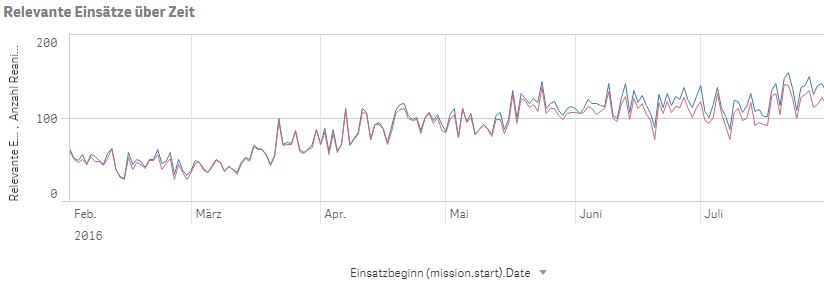
\includegraphics[width=1\linewidth]{img/konzcomp1}  
%  \caption{Darstellung des Liniendiagramms mit der tatsächlichen Datumsangabe}
%  \label{fig:komp1}
%\end{subfigure}
%\begin{subfigure}{0.5\linewidth}
%  \centering
%  % include second image
%  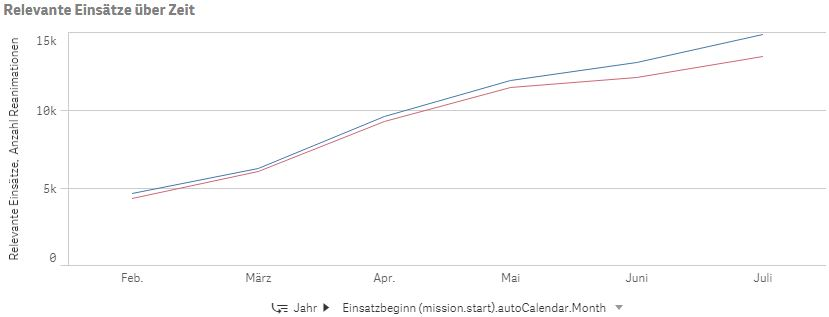
\includegraphics[width=1\linewidth]{img/konzcomp2}  
%  \caption{Gleiche Daten mit einer Aggregation auf Jahr-Monat}
%  \label{fig:komp2}
%\end{subfigure}
%\caption[Vergleich zwischen den unterschiedlichen Dimensionen]{Vergleich zwischen den unterschiedlichen Dimensionen}
%\label{fig:compDim}
%\end{figure}

Die Aufsummierung in Monate, alternativ auch Wochen, bringt je nach Datenlage eine recht glatte Kurve mit sich. 
Die Kennzahlen dieser Visualisierung sind die Summe der relevanten Einsätze und zum Vergleich die Summe der Reanimationen. 
Eine Mini-Legende unterhalb der Grafik erleichtert die Orientierung, sollte der Nutzer in einen bestimmten Zeitraum "`reinzoomen"'.

%Es wurde die AutoCalendar-Funktion genutzt, damit ein fließender Übergang zwischen den Jahren möglich ist.

Darunter sind zwei Kreisdiagramme zu sehen (3, 4), welche die Anzahl der Einsätze und der Reanimationen pro Gerätetyp anzeigen.
Diese Art der Visualisierung wurde gewählt, damit die Relation und Verteilung unter den Geräten deutlich gemacht wird.
Unter dem jeweiligen Kreisdiagramm ist als einzelner \gls{KPI} die durchschnittliche Einsatz- und Reanimationsdauer.

%\bildrechts
%{filter}
%{4cm}
%{Gleichbleibendes Filterfenster auf den jeweiligen Dashboards}
%{filt}

\label{par:filter}
Außerdem soll der Nutzer auf jedem Arbeitsblatt die Möglichkeit haben, die wichtigsten Filter jederzeit und schnell benutzen zu können.
Hierfür wird, wie es in der Regel bei Nutzern von PC- und Web-Applikationen im mentalen Modell erwartet wird \cite{Grunwied.2017}, auf der linken Seite ein gleichbleibender Bereich für die Filteroptionen angelegt (5).
Die häufigsten und essentiellen Optionen sind hierbei Zeit mit Jahr, Monat, Woche, Wochentag und die Geräte als \gls{Drilldown} mit Typ und anschließend der Seriennummern, zu sehen auf der linken Seite in Abbildung \ref{fig:einsatzzeitpunkt}.

\subsubsection{Einsatzzeitpunkt}
\label{subsub:zeitpunkt}
\bildbreit
{einsatzzeitpunkt}
{Dashboard zu den Einsatzzeitpunkten}
{Prototyp Einsatzzeitpunkt-Visualisierung}

Es gibt eine Vielzahl and Fragestellungen zu den Einsatzzeitpunkten. (\todo{Beispiele})
Das Arbeitsblatt in Abbildung \ref{fig:einsatzzeitpunkt} soll einen Überblick geben, zu welchen Tages- und Uhrzeiten die Einsätze stattfinden.
Hierbei gibt es drei verschiedene Detailstufen: Tageszeit (1), stündlich (2) und halbstündlich (3). 
So kann der entsprechende Nutzer für seinen Bedarf die jeweilige Auslastung oder Einsatzhäufigkeit herausfinden.
Des Weiteren sind unten, unterhalb der Tageszyklen (Tageszeit und Stunden), zwei weitere Diagramme, welche die Anzahl der Einsätze und Reanimationen für Wochentage (4) und Monate (5) anzeigt. 
Somit ist jeder relevante zeitliche Zyklus abgedeckt und es können Auswertungen beispielsweise zu Tageszeiten wie nachts, Wochentage wie Wochenende oder saisonalen Zeiträume vollzogen werden.

Es wurden zur Darstellung Kombi-Diagramme gewählt, um normale Einsätze und Reanimationen getrennt, aber dennoch in Relation betrachten zu können.
Die Balken eignen sich gut, um das Volumen eines Zeitpunktes mit anderen leicht vergleichen zu können und repräsentieren die Menge an relevanten Einsätzen.
Die Anzahl der Reanimationen wurde als Linie mit einer alternativen Y-Achsen-Skalierung visualisiert, damit auch geringe Vorkommen, wie in der Praxis häufig der Fall, noch gut sichtbar sind, da die obere und untere Grenze unabhängig der Anzahl aller Einsätze ist.
Würde man diese als Balken neben die normalen Einsätze legen, wären sie kaum zu sehen und Unterschiede zwischen den jeweiligen Zeitpunkten wären nur schwer zu erkennen.
Mit der alternativen Liniendarstellung ist die untere Kante der X-Achse nicht immer 0, wie es bei der Darstellung von Balken der Fall ist, sondern kann beim Minimum der entsprechenden Kennzahl beginnen.
%Timebuckets wurden selber geskriptet, damit nicht zu fein nach minute ?

\subsubsection{Einsatzdauer}
\label{subsub:dauer}
\bildbreit
{einsatzdauer}
{Dashboard zu der Dauer von Einsätzen}
{Prototyp Einsatzdauer-Visualisierung}

Die Dauer von Einsätzen ist ebenfalls eine gefragte Information. \todotext{ref}
\todotext{Beispiele: Hierbei sind Fragen wie }
Je nach entsprechenden Vorgaben können hierbei unterschiedliche Auswertungen durchgeführt werden.
Sollen die Rettungskräfte beispielsweise das Gerät immer sofort beim Losfahren starten, können gegebenenfalls Auswertungen zu den Fahrtzeiten getroffen werden.
Oder wenn das Personal das Gerät erst vor Ort anschalten soll, kann die tatsächliche Einsatzzeit verglichen werden.
Es kommt also auf die Vorgaben der entsprechenden Instanzen drauf an, welche Analysen durchgeführt werden können.

Als generelles Modell werden auf diesem Dashboard, in Abbildung \ref{fig:einsatzdauer} zu sehen, die grundlegenden Informationen zur Dauer dargestellt.
Dazu zählt die globale durchschnittliche Missionsdauer (1), sowie die absolute Gesamteinsatzdauer (2), welches unter anderem eine durch die Bundeswehr gefragte \gls{KPI} ist.
Des Weiteren gibt es die mittlere Einsatzdauer nach Gerätetyp aufgeschlüsselt (3). 
Dies ist zugehörig unter der Geräteübergreifenden \gls{KPI} als Balkendiagramm dargestellt, damit die Werte gut miteinander vergleichbar sind.


Darunter sind zwei weitere Diagramme zu finden, welche als Histogramm\footnote{\glqq grafische Darstellung einer Häufigkeitsverteilung in Form von Säulen, die den Häufigkeiten der Messwerte entsprechen\grqq{} \cite{Dudenredaktion.2015}} die Häufigkeit verschiedener Einsatz- (4) sowie \gls{CPR}-Dauer (5) darstellen.
%\bildrechts{Dauer-klasse} {5cm} {w} {wa}
Dabei werden je nach maximaler Dauer dynamisch gleichgroße Bereiche oder \glqq Klassen\grqq{} definiert.
So gibt es beispielsweise den Bereich \glqq 0 <= Reanimationsdauer in Min. < 16\grqq{}, welcher hier >4000 Einsätze zählt, danach Reanimationsdauer größer gleich 16 und kleiner als 32 mit ca. 400 Missionen.
Dies wird in diesen 16-Minuten-Schritten\footnote{Diese Einteilung basiert auf einer Berechnung von Minimum, Maximum und einer präferierten Anzahl an Balken.
In diesem Beispiel ist das Minimum = 1, Maximum = 220 und die präferierte Anzahl an Balken ist standardmäßig 14.
Daraus ergibt sich folgende Berechnung: $\frac{Maximum-Minimum}{Anzahl Balken}$ = $\frac{220-1}{14}$ $\approx$ 16}
 weiter bis zur maximal vorhandenen Reanimationsdauer fortgeführt.
Dabei wird die Verteilung von Einsätzen und Reanimationen mit einer entsprechenden Dauer sichtbar und es können weiterführende Analysen auf Basis der Einsatzdauer vorgenommen werden.

\subsubsection{Geräte}
\label{subsub:geräte}
\bildbreit
{devices}
{Dashboard zu den entsprechend vorhandenen Geräten}
{Prototyp Geräte-Visualisierung}

\todo{Photoshop Number! WRONG}
Das folgende in Abbildung \ref{fig:devices} präsentierte Arbeitsblatt gibt dem Nutzer eine Übersicht seiner eingesetzten Geräte.
Dabei gibt es die eindeutige \gls{KPI} \glqq Anzahl Geräte\grqq{} (1), welche die distinkten Geräte zählt, von denen bis dato Missionen in dem vorliegenden \gls{ANALYSE}- Server vorliegen.
Sofern der entsprechende Betreiber den Upload oder das nachträgliche Importieren der Einsätze auf den Server anordnet, kann hiermit die gesamte Anzahl an Geräten überwacht werden. %(Aktive Geräte? bsp Einsatz in letztem quartal? In umsetzung aufnehmen)
Ergänzend zu dieser pauschalen Zahl gibt es in intuitiver Leserichtung rechts eine Visualisierung, wie viele Geräte einer Art vorliegen (2).
Die Art der Darstellung ist ein Kreisdiagramm, da in der Regel eine Geräteart überwiegen wird, und somit diese in Relation zu der Gesamtheit gesetzt wird.

Darunterliegend finden sich zwei Balkendiagramme wieder, welche die Anzahl der Einsätze und Reanimationen nach den einzelnen Geräten mittels Seriennummer (3) und/oder Geräte-ID (4) aufschlüsseln.
Dies präsentiert die Einsatzhäufigkeit von den Einzelgeräten und kann dadurch beispielsweise als Grundlage für Schichtplanung oder Neuanschaffung von Geräten dienen.

\subsubsection{Reanimation}
\label{subsub:reanimation}
\bildbreit
{reanimation}
{Dashboard zu den Daten des \gls{CPR-Feedbacksensor}s}
{Prototyp Reanimations-Visualisierung}

Die nachträgliche Auswertung einer Reanimation ist für viele Stakeholder eine wichtige Aufgabe.
Dabei gibt es beispielsweise die klassische Nachbesprechung zwischen Notfallsanitäter und Auszubildenden oder aber auch die medizinische Forschung, welche Ereignisse und Werte einer Reanimationen untersuchen um gegebenenfalls neue Erkenntnisse zu gewinnen.
Eine Analyse über viele Reanimationen hinweg ist hierbei für viele Nutzergruppen ein neuer Weg, welcher bisher unentdeckte Zusammenhänge offenbaren oder bereits angenommene Hypothesen bestätigen kann.

Ein wichtiger Erfolgsfaktor einer Reanimation ist eine adäquate Drucktiefe, welche zwischen 5-6cm liegen soll  \cite{Monsieurs.2015}.
Sofern ein \gls{CPR-Feedbacksensor} bei einer Reanimation verwendet wird, kann die Drucktiefe jeder Kompression eingesehen werden. %(auch vorOrtFeedback)
Eine Auswertung zur Tiefe über viele Reanimationen hinweg kann im obersten Balkendiagramm (1) in Abbildung \ref{fig:reanimation} betrachtet werden.
Dabei sind horizontal die verschiedenen Drucktiefen und vertikal die Anzahl der Missionen mit dieser Tiefe angeordnet.
Die Farbgebung mit rot und grün soll dem Benutzer helfen, schnell die \glqq guten\grqq{} Kompressionen von den unzureichenden zu unterscheiden.

Ein wichtiger Punkt hierbei ist, dass derzeit pro Reanimation genau ein Durchschnittswert der Drucktiefe gebildet wird und zum Export bereitsteht.
Es ist somit eine stark voraggregierte Information, welche einen eventuellen falschen Wert widerspiegelt. 
So kann beispielsweise eine Reanimation 100 zu flache Kompressionen mit 4cm, sowie 100 zu tiefe Kompressionen  mit 7cm enthalten.
Der nun aggregierte Mittelwert dieser Reanimation lautet 5,5cm und suggeriert eine an der Drucktiefe gemessene, \glqq perfekte\grqq{} Reanimation, obwohl nicht eine korrekte Kompression vorliegt.
Dieser Aspekt muss bei der Betrachtung dieser Auswertung berücksichtigt werden.
Eine mögliche Lösung oder zum Mindesten eine Verbesserung der Aussagekraft zur Drucktiefe wird in Kapitel \ref{sub:erweiterung} beschrieben.

Zur rechten Seite der oben beschriebenen Visualisierung ist ein Boxplot-Diagramm (2), welches eine Zusammenfassung zur Drucktiefe liefert.
Es zeigt kompakt die maximale und minimale durchschnittliche Tiefe, sowie die Quartile und den Median aller Reanimationen an.

Des Weiteren sind drei Diagramme (3, 4) vorhanden, welche mehr die Funktion von Platzhaltern einnehmen, da es zur Druckfrequenz und \gls{CCF} zum Zeitpunkt dieser Konzeption keine aussagekräftigen Daten gab.
Dennoch ist es eine sehr relevante und gefragte Information und soll in \ref{sub:erweiterung} weiter betrachtet werden.


\subsubsection{Defibrillationen}
\label{subsub:schocks}

\bildbreit
{shocks}
{Dashboard zu den abgegebenen Defibrillationen}
{Prototyp Defibrillations-Visualisierung}

Ergänzend zu den in \ref{subsub:reanimation} beschriebenen Reanimationen sind auch die Defibrillationen oder \glqq Schocks\grqq{} von Relevanz.
Denn jeder Einsatz mit Schockabgabe ist eine Reanimation, doch konträr beinhaltet nicht jede Reanimation Defibrillationen.

Die Abbildung \ref{fig:shocks} zeigt das dazugehörige Arbeitsblatt.
Als generelle Statistik gibt es die Anzahl der Einsätze mit Schockabgabe (1), wie auch die Gesamtzahl  und durchschnittliche Zahl pro Einsatz abgegebenen Defibrillationen (2).
Daneben gibt es ein Kreisdiagramm (3), welches sich hervorragend für den Vergleich von binären Optionen eignet, da die entsprechenden Anteile sofort ersichtlich werden.
Hierbei werden die zwei Möglichkeiten der Schockabgabe verglichen: \gls{AED} und Manuell.
Als weitere \gls{KPI} ist ergänzend dazu die Anzahl der Wechsel zwischen den Defibrillationsmodi (4).

Darunter findet sich ein Balkendiagramm wieder, welches die Anzahl der Schocks nach jeweiliger eingestellter Energie in Joule darstellen soll (5).
Zum Zeitpunkt dieser Konzeption war dies nicht möglich, da die Schocks wie auch die Kompressionen des Feedbacksensors nicht einzeln vorliegen, sondern voraggregiert werden und somit nur Min- und Max-Werte vorliegen.
Da die Defibrillation eine aufschlussreiche Informationsquelle sind, wird eine Lösung in \ref{sub:erweiterung} weiter erarbeitet.

Eine Besonderheit bei der Visualisierung ist, dass die Defibrillationen, welche mit 200J abgegeben wurden, ausgeschlossen werden.
Dies hat den Hintergrund, dass dies der voreingestellte Default-Wert und somit der überwiegende Teil aller Schocks mit dieser Energiemenge abgegeben werden.
Würde man diesen Wert nicht ausschließen, führt das dazu, dass die restlichen \glqq Rand\grqq{}-Werte untergehen und in der Grafik kaum oder gar nicht sichtbar sind.

Eine weitere Information ist am unteren Ende des Arbeitsblattes zu finden (6).
Dort werden aufgeschlüsselt nach den einzelnen Geräten die insgesamt abgegebenen Defibrillationen angezeigt.
%Somit (Fragestellungen?) können Auswertungen gemacht werden, welches Team/Wache/Fahrzeug wie viele Schocks abgegeben hat etc.
%Shock mit Zeitverlauf! Monat... | Prozent von allen Einsätzen

\subsubsection{Blutdruck}
\label{subsub:nibd}
\bildbreit
{nibd}
{Dashboard zu den Blutdruckmessungen}
{Prototyp Blutdruck-Visualisierung}
%nibd, leider nur min max avg, keiine einzel messungen, gefordertes neues Modell, wie in kap 123 beschrieben 

Ein weiterer möglicher Bestandteil einer Mission ist die \gls{NIBD}.
Die zugrundeliegenden Daten sind auch bei diesem Segment vorab zusammengefasst.
Somit ist lediglich die Anzahl der Messungen und die maximale Messdauer pro Mission verfügbar.
Um auch hier wirksame Analysen und Auswertungen möglich zu machen, werden in \ref{sub:erweiterung} Ansätze zur Bereitstellung von den einzelnen Messungen verfolgt.

Aus den bis dato vorliegenden Daten wurden drei \gls{KPI}s und ein Balkendiagramm extrahiert:
Anzahl der Einsätze, die eine \gls{NIBD}-Messung hatten (1), die Gesamtanzahl der Messungen (2) und daraus errechnet der Durchschnitt der Messungen pro Einsatz (3).
Das Balkendiagramm stellt die Anzahl der Messungen nach maximaler Messdauer dar (4).
Mit der Tabelle (5) können die jeweiligen Einsatz-UUIDs und \gls{NIBD}-Statistiken betrachtet werden. 



\subsubsection{Weitere}
\label{subsub:weitere}
Die folgenden Elemente wurden als \glqq Weitere\grqq{} zusammengefasst, da die Datenlage voraussichtlich recht wenig sein wird und die Nachfrage nicht sehr groß, aber dennoch vorhanden ist.

%\bildrechts
%{sensorik2}
%{3cm}
%{Kreisdiagramme der Sensorik}
%{Sensorik-Visualisierung}
%\FloatBarrier

So spielt die Sensorik zum Beispiel doch eine große Rolle. 
Das Dashboard als solches bietet keine großen Diagramme oder neue Erkenntnisse, dennoch soll es einen Überblick schaffen.
Kreisdiagramme, wie in Abbildung \ref{fig:sensorik2} zu sehen, sind hier eine gute Wahl aufgrund der binären Optionen, ob eine Sensorik verwendet wurde oder nicht.
Auch bieten sie als Filter eine nützliche Funktion, wenn beispielsweise Reanimationen gezeigt werden sollen, bei den sowohl ein Ruhe-EKG als auch CO2 gemessen wurde.

Des Weiteren gibt es auch Patientendaten, welche manuell oder durch die Krankenversicherten-Karte in dem \gls{C3} eingetragen werden können.
Die auswertbaren Daten hierbei sind Alter, Geschlecht und Herkunft, wobei Herkunft in der Praxis fast nie gepflegt wird und für eine Auswertung auch keine große Relevanz darstellt.
Alter und Geschlecht sind jedoch sehr spannende Daten, welche in Kombination mit anderen Metriken spannende Auswertungen liefern kann.
Dabei ist eine Darstellung des Medians des Alters sinnvoll. 
Ob dies mit einem Boxplot-Diagramm oder einer \gls{KPI} und ergänzend ein Histogramm dargestellt wird, soll später erörtert werden.
Zuerst muss hierbei auch der Aspekt der Anonymisierung betrachtet werden. 
Dies kann in \ref{sub:recht} nachgelesen werden.
Das Geschlecht kann aufgrund der wenigen Optionen gut als Kreisdiagramm dargestellt werden.

Zum Schluss gibt es noch einige wenige Daten zu dem \gls{pacer}.
Aufgrund der seltenen Einsatzhäufigkeit bei Rettungseinsätzen steht die Implementierung dieses Dashboards noch zur Frage offen.
Mögliche Informationen wären die Anzahl der Missionen mit Pacer-Einsatz und in welchem Modus. 
Andere interessante Daten wie in Anhang \ref{fragestellungenPacer} beschrieben sind zu diesem Zeitpunkt nicht exportierbar und das Entwickeln dieser Funktionalität ist aufgrund des seltenen Einsatzes derzeit unwahrscheinlich.

%\section{Generierung von Dummy-Daten?}
% Kap. Umsetzung?

\section{Evaluierung  des Prototypen}
\label{sec:evaluierung}
\subsection{Vorgehen bei der Prototyp-Evaluierung}
\label{sub:vorgehenEvaluierung}
Zur Evaluierung des Prototyps werden vorerst, wie in \ref{sec:vorgehenKonzept} beschrieben, firmenintern geeignete Personen gesucht. 
Dabei wurden Mitarbeiter aus den Abteilungen Medizinische Forschung und Anwendung, Applikations- beziehungsweise Anwendungsspezialisten und Produktmanagement gewählt, da hier ein guter/großer Praxisbezug herrscht und die Erfahrungen, Wissen und Anforderungen ähnlich zu denen der zukünftigen Kunden sind.

%\citeDürrenberger für Fokusgruppen!!

Für die Evaluierung wurde eine abgewandelte Form der klassischen Fokusgruppen-Evaluation angewandt  \cite{Christoforakos.2017}.
Hierbei wird eine kleinere Gruppe von Teilnehmern zusammengestellt, welche die voraussichtlichen Kunden generell abbilden soll. 
Danach ist es im Grunde genommen eine offene Gruppendiskussion, welche durch einen Moderator geleitet wird, sodass der entsprechende Fokus nicht außer Acht gelassen wird und etwaige Diskussionen und Gedankenaustausche in die richtige Richtung gelenkt werden \cite{Durrenberger.1999}.
In diesen Evaluierungen spielt die Beobachtung der Teilnehmer keine große Rolle, wie normalerweise in den meisten Fokusgruppen üblich, da sie dass System als solche nicht bedienen und in diesem Fall aus der Beobachtung keine großen Erkenntnisse gewonnen werden können.

Die Vorteile einer Fokusgruppe sind, dass sich Personen in diesem Gebiet bereits auskennen und direktes Feedback geben können. 
So ergibt sich in relativ kurzer Zeit eine große Datenmenge und kritische Rückmeldungen zum Prototyp, welche bei Bedarf im gleichen Zug weiter ausgeführt und/oder diskutiert werden können.
Auch möglicherweise auftretende Fragen von den Personen können, im Gegensatz zu reinen Umfragen, direkt beantwortet werden um so Missverständnisse und Unklarheiten aufzuklären.

Für die Evaluierung wurde eine Gruppengröße von ca. 3-4 Personen gewählt, was etwas unter der üblichen Fokusgruppengröße von ca. 6-8 Personen liegt (vgl. \cite{Madche.}). 
Grund hierfür sind zum einen die erwünschten 3-4 unterschiedlichen Gruppen, welche bei den ca. 16 geeigneten Personen diese Gruppengröße vorgibt, zum anderen ist es auch von Vorteil was das Einbringen von Ideen und Kritik von jeder Einzelperson angeht.
Dennoch kann ein fachlicher Austausch zwischen verschiedenen Personen stattfinden, welcher für weiterführende Diskussionen sehr hilfreich sein kann. 

Bei der Einteilung der Personen in die jeweiligen Fokusgruppen wurde auf verschiedene Eigenschaften und Bedingungen, wie zum Beispiel Alter, Abteilung, Wissenstand, Erfahrungen, und vieles mehr geachtet. 
Ziel waren einerseits homogene Gruppen, wo die Personen ähnliche Hintergründe und Altersklassen haben, andererseits sollte auch eine gewisse Heterogenität herrschen, damit verschiedene Meinungen aufeinander treffen und kontroverse Diskussionen angeregt/gefördert werden.
So ist beispielsweise eine Gruppe von eher jungen medizinischen Forschern in einer ähnlichen Altersklasse zwischen 23-27 Jahren, aber mit verschiedenen Hintergründen, beziehungsweise Spezialisierungen zu Informatik, Rettungsdienst und medizinische Studien und Auswertungen.

Mit der kleineren Größe der Gruppe wurde auch ein etwas kürzerer Zeitraum der jeweiligen Evaluierung gewählt.
Demnach liegt sie (des Öfteren) bei einer Gruppe von 6-8 Personen bei ca. 90 Minuten (vgl. \cite{Madche.}) und für die hier durchgeführten Termine wurden 60 Minuten angesetzt, was pro Person gerechnet sogar etwas mehr Zeit ist.
Jedoch ist diese Rechnung/Vergleich nicht repräsentativ und daher mit Vorsicht zu betrachten.

Es werden die erstellten Dashboards aus \ref{sub:erstellungDashboards} in der Gruppe vorgestellt. 
Dabei wird anfangs den Personen erläutert, was der Sinn und Zweck der Visualisierungen ist und für welche Endnutzer er von Relevanz sein wird.
Somit können sie sich in die Lage der Kunden versetzen und aus deren Perspektive die präsentierten Ergebnisse kritisch betrachten.

Anschließend wird jedes Arbeitsblatt präsentiert, gefolgt von einer kurzen Pause, damit sich der erste Eindruck bilden kann und darauffolgend eine kurze Einführung/Erklärung zum aktuellen Fenster geliefert, um eine einheitliche Diskussionsbasis zu schaffen.
Des Weiteren wurden Hand-Outs ausgehändigt, damit jede Person zu jeder Zeit jedes Dashboard vor sich liegen hat um gegebenenfalls Anmerkungen, Kommentare, Verbesserungsvorschläge, Fragen oder ähnliches an die entsprechende Stelle notieren zu können.
Im Laufe der Zeit wurden eingebrachte Ideen umgesetzt und den Personen als Alternative vorgesetzt.
So konnten die zwei Versionen direkt miteinander verglichen werden und ähnlich wie bei einem A/B-Test die bessere Alternative weiter verfolgt werden.
Dies hat den weiteren Vorteil, dass es zur Nachbereitung verwendet werden kann, da die Gedanken und Ideen der Teilnehmer im Nachhinein dokumentiert zur Verfügung stehen und weitere Schritte oder Änderungen darauf basierend vorgenommen werden können. 
Ein Auszug dieser Hand-Outs kann im Anhang \ref{att:evaluation} betrachtet werden.

Die beschriebenen Diagramme oder dargestellten Abbildungen können von Kapitel \ref{sec:erstellungPrototyp} abweichen, da im mehrstufig-iterativen Prozess immer Änderungen durchgeführt wurden und somit keine zeitliche Reihenfolge gegeben ist.
In den folgenden Kapiteln wird nur ein Auszug der Gruppen und dort jeweils ausgewählte prägnante Kritik oder Änderungsvorschläge genannt.
Es wurden viele Variationen, neue Dashboards, andere Visualisierungen, Textvariationen und vieles mehr probiert, all diese aufzuzeigen würde den Rahmen des Kapitels überziehen.

\subsection{Gruppe 1: medizinische Forschung und Anwendung}
\label{sub:gruppe1}
% Gruppenbeschreibung?
Ein erster und von der Gruppe einstimmiger Fehler war ein Element der Filterleiste an der linken Seite der meisten Dashboards.
Hier war die Sortierung der Wochentage teilweise in alphabetischer Reihenfolge, statt chronologisch Montag - Dienstag...
Dies war ein Fehler, welcher durch inkonsistente Datengrundlage der unterschiedlichen Geräte eintrat, so waren die Wochentage des \gls{cCPR} und \gls{LIVE} rechtsbündig angelegt und somit für Qlik nicht als Datum auswertbar.

Des Weiteren wurde für die Filterliste vorgeschlagen, nach der jeweiligen \glqq Device-ID\grqq{} filtern zu können.
Diese Funktion war bereits teilweise implementiert, jedoch als verstecktes \gls{Drilldown} nach Auswahl einer Geräteart und anschließend konnte nach technischer Seriennummer gefiltert werden.
Dies wurde in der Gruppe weiter diskutiert, doch eine Filterung nach Geräte-ID scheint sinnvoller zu sein.

In Bezug zu den Filtern kam außerdem die Idee, feste vordefinierte Filter vorzugeben.
Beispielsweise \glqq Alle Reanimationen die letzten Monat in der Nacht stattfanden\grqq{}. 
Qlik Sense bietet eine solche Funktionalität unter dem Namen \glqq Lesezeichen\grqq{}, welche getätigte Markierungen und Filter unter einem Namen speichert.
Da mit den Kombinationsmöglichkeiten eine sehr große Anzahl solcher definierter Lesezeichen entstehen kann, ist es vermutlich sinnvoll, diese Funktion dem jeweiligen Nutzer zur Verfügung zu stellen.
Dies sollte im Funktionsumfang beim Lizenzierungsmodell mit den zugehörigen Funktionen beachtet werden.

Die Gruppe legte auch großen Wert auf Nutzerführung.
Die ersten Titel der jeweiligen Diagramme waren oft unzureichend formuliert und haben dem Nutzer zu wenig Informationen gegeben, um die Visualisierung schnell zu verstehen.
Auch Informationen beim \glqq \gls{Hovern}\grqq{} oder als zusätzlicher \gls{Button} wären hilfreich, um gegebenenfalls komplexere Diagramme weiter zu erläutern und die zugrundeliegenden Daten zu beschreiben. 
Insgesamt spielt die Usability eine große Rolle und sollte bei der Umsetzung starke Beachtung bekommen.

Als Einstiegspunkt und Übersicht in das Programm soll das erste Arbeitsblatt dienen.
Hier ist die Gruppe der Meinung, dass je nach Zielgruppe eine unterschiedliche Startseite Sinn macht.
So wäre für den Rettungswachenleiter als Erstes andere Zahlen interessant, wie für ein Mitarbeiter des Qualitätsmanagement.
%Etwaige Startseiten werden in Kap\ref{zielgruppStartseite} weiter erläutert.

Die zu evaluierende Startseite hatte ein ähnliches Diagramm wie \ref{fig:Uebersicht_Prototyp} (siehe Anhang \ref{att:evaluation}).
Hierbei war der Vorschlag, das linke Wasserfall-Diagramm in zwei Diagramme aufzuteilen, da sie zum einen die Einsätze und zum anderen die Reanimationen kategorisieren.
Generell war der Vorschlag, eine Einsatz-Startseite und eine ähnliche nur für Reanimationen zu gestalten, da auch die durchschnittlichen Zeitspannen von Einsatz und Reanimationsdauer in keinem direkten Verhältnis stehen.
% Ein weiterer Vorschlag war, eine Startseite mit den aktuellsten Meldungen zu erstellen. Hierbei sollen zb die von letztem Tag, woche monat, dargestellt werden. (Umsetzung/Startseite...)

Beim Dashboard Einsatzzeitpunkt, siehe \ref{subsub:zeitpunkt}, wurde bemerkt, dass die Tagesabschnitte eine unterschiedliche Anzahl an Stunden haben. 
So hat der Morgen fünf, der Mittag sieben und Abends und Nachts jeweils sechs Stunden.
Dies rechnet Einsätze, die für den Morgen kategorisiert werden sollten, zu den Mittags-Einsätzen hinzu und verfälscht somit den Eindruck.
Des Weiteren wurde erfragt, in welchem Detailgrad die Auswertung Sinn macht.
Dabei kam in der Diskussion heraus, dass nicht alle drei Diagramme zu sehen sein müssen. 
Je nach Anwender ist ein unterschiedlicher Detailgrad von Relevanz, sodass es im besten Fall konfigurierbar sein sollte.% \ref{Internatio?}.
Auch die Darstellung von Reanimationen als Linie im Kombinations-Diagramm schien für die Gruppe verwirrend.
In späteren Evaluierungen wurde die vorgeschlagene Alternative, die Reanimationen als zweiten Balken nebeneinander darzustellen, präsentiert und stellte sich jedoch als eher unbrauchbar heraus.

%\bildrechts
%{radar}
%{8cm}
%{Radar-Chart Visualisierung der Einsatzzeitpunkte}
%{Prototyp Einsatzzeit-Alternative}

\bildbreit
{radar}
%{8cm}
{Radar-Chart Visualisierung der Einsatzzeitpunkte}
{Prototyp Einsatzzeit-Alternative}

Eine Erweiterung des in Kapitel \ref{sec:erstellungPrototyp} präsentierten Prototyps war die Darstellung der Einsatzzeitpunkte (siehe Kapitel \ref{subsub:zeitpunkt}) als Radar-Chart\footnote{Ein Radar-Chart (Radar-Diagramm) zeigt in radialer Form die Ausschläge von Daten.
Es ist im Prinzip ein Liniendiagramm, welches am Anfang mit dem verbunden ist.
Voraussetzung hierfür ist demnach eine zyklische Datengrundlage, welche sich wiederholen muss.
Da sich fast alle Zeitdaten zyklisch darstellen, ist es eine gute Visualisierung solcher Daten.

Die Namensgebung kommt von der Ähnlichkeit mit einem Radarmonitor beispielsweise in einem U-Boot oder  Schiff.}.
Diese eignen sich sehr gut, um zyklische Daten wie Wochentage, Uhrzeiten, Monate zu visualisieren.
Da dies keine offizielle Erweiterung von Qlik Sense ist, ist die Funktionalität nicht zu einhundert Prozent gewährleistet.
Dennoch kam die Visualisierung gut bei der Gruppe an und ein Use-Case wäre beispielsweise der Vergleich der Auslastung von zwei Wachen, indem man etwa zwei oder mehrere Geräte-IDs auswählt.
Die fehlerfreie Darstellung müsste jedoch weiter getestet werden.

Bei dem Dashboard zu der Dauer von Einsätzen kam der Vorschlag auf, das Histogramm der Dauer logarithmisch darzustellen.
Der Unterschied ob ein Einsatz zwei oder drei Minuten lang ging gegenüber 64 oder 65 Minuten sei mit einer logarithmischen Darstellung besser, war die Argumentation.
Außerdem ist bei der Gesamteinsatzdauer keine Legende, wodurch nicht erkennbar ist, ob es sich bei der ersten Zahl um  Tage oder Stunden handelt.

Das Balkendiagramm zu der Schockenergie, in Abbildung \ref{fig:shocks} zu sehen, war ein weiterer Diskussionspunkt.
Eine Anmerkung hierzu war, dass die X-Achsen-Skala kontinuierlich sein soll. 
Zum Zeitpunkt der Evaluation wurden nur alle vorhandenen (außer 200J) eingestellten Energiestufen abgebildet.
Wenn es fünf Stufen unter und 15 Stufen über 100J gab, erweckte das Diagramm den Eindruck, dass es viel weniger Schocks unter 100J gab.
%Bild zur Klärung?
Doch besteht die Möglichkeit, dass in den fünf Energiestufen viel mehr Schocks abgegeben wurden, als in den 15 Stufen über 100J.
Des Weiteren sollte es eine \gls{KPI} zu der Anzahl der Schocks geben, die 200J als Energie hatten.
Ergänzend dazu wären auch die Summe aller Schocks, die nicht 200J hatten, als eigenständige Kennzahl denkbar.

Als generelles Feedback dieser Gruppe wurde auch ein Übermaß an Informationen bei manchen Dashboards genannt.
Eine Aufteilung von einem Dashboard in zwei oder mehrere sei hier denkbar.
% Auch wurden viele positive Aspekte genannt und gelobt.

\subsection{Gruppe 2: Applikationsspezialisten}
\label{sub:gruppe2}
Dieser Zusammenschluss von Anwendungsspezialisten hatte auch, wie die Gruppe in \ref{sub:gruppe1}, angemerkt, dass eine zielgruppenspezifische Startseite Sinn machen würde.
Des Weiteren wurde das überarbeitete Wasserfalldiagramm aus Abbildung \ref{fig:Uebersicht_Prototyp} kommentiert. 
Demnach sei die grafische Kategorisierung der Einsätze und Reanimationen nicht zwingend erforderlich, da eine einfache Prozentangabe ausreichend wäre (Beispiel: 120 Einsätze, 12\% Reanimationen).
Das Kreisdiagramm muss laut den Spezialisten keine Dimensionierung nach allen Gerätearten vornehmen, sondern ein direkter Vergleich zwischen \gls{cCPR} und Standard-Defibrillatoren  (\gls{C3}, \gls{C1}) sei ebenfalls ausreichend.

In den Sitzungen mit dieser Gruppe war die Frage nach Klassifizierung einer Reanimation ein öfter auftretender und relevanter Bestandteil.
Sobald der \gls{CPR-Feedbacksensor} verwendet wurde, ist es, sofern kein Puppen- oder Testeinsatz, mit hoher Wahrscheinlichkeit eine Reanimation.
Alle anderen Wiederbelebungen müssen mittels prägnanter Ereignisse ermittelt werden. 
So ist die Abgabe von Defibrillationen ein guter und verlässlicher Indikator für eine Reanimation.
Sollte allerdings eine Reanimation ohne Feedbacksensor und ohne Schockabgabe erfolgen\footnote{Nicht jeder Herzstillstand ist Defibrillationspflichtig \cite{Nolan.2010}}, fällt sie zum derzeitigen Zeitpunkt in die Kategorie \glqq sonstiger Einsatz\grqq{}
So wurde über Ereignissen überlegt, welche eine Reanimation kennzeichnen.
Beispiele hierfür waren unter anderem das Öffnen des Defibrillations-Menüs, Starten einer Analyse, Kleben von den Defibrillations-Elektroden.
Inwiefern diese Ereignisse zum diesem Zeitpunkt zur Auswertung zur Verfügung stehen, muss geklärt werden. %Kap\ref{kapReaErkennung}

Auch der Aspekt der Qualitätssicherung im Rahmen einer Reanimation spielt laut der Gruppe eine große Rolle.
Demnach wäre ein zusätzliches Dashboard interessant, aus welchem hervorgeht, ob geforderte Maßnahmen durchgeführt wurden.
Beispielsweise ob währenddessen eine \gls{Kapnografie} durchgeführt wurde oder ob, und wenn ja wie ein EKG mit STEMI\footnote{STEMI steht für \glqq ST-elevation myocardial infarction\grqq{} und bezeichnet üblicherweise einen Herzinfarkt, welcher durch die Hebung der ST-Strecke in einem EKG klassifiziert wird \cite{Horacek.1998}} übertragen wurde.
Ebenso wäre aufschlussreich, wie der erste Rhythmus war. 
Ob dies umzusetzen ist, ist fraglich und zum derzeitigen Zeitpunkt eher unwahrscheinlich.

\label{par:binning}
Bei der Darstellung der Reanimationsqualität, siehe Abbildung \ref{fig:reanimation}, gab es die Vorschläge, nicht jeden einzelnen Wert präzise zu präsentieren, sondern ein \glqq \gls{Binning}\grqq{} durchzuführen.
Argumentation hierfür war, dass es irrelevant ist, ob die Drucktiefe 1.2 oder 1.3cm war, interessanter ist wie viele es zwischen 1-2cm oder gar 1-3cm gibt.
Gleiches Prinzip gilt auch bei der Druckfrequenz.

Auch eine Darstellung der Einsätze nach Ort wäre laut den Personen sehr interessant.
Diese Umsetzung ist jedoch fraglich, beziehungsweise müsste es draußen im Einsatz gepflegt werden, was stand heute nicht der Realität entspricht.
In Zukunft soll jedoch die Möglichkeit bestehen, die Einsätze mit Dokumentationssystemen, wie dem NIDA-Pad, zu kombinieren.
Dies würde zu einer Vielzahl neuer möglicher Auswertungen führen, unter anderem der Ort des Einsatzes.

\subsection{Gruppe 3: Produktmanagement und medizinische Forschung und Anwendung}
\label{sub:gruppe3}

In dieser Gruppe kamen den Personen die neu hinzugefügten Radar-Diagramme, siehe Abbildung \ref{fig:radar}, im Gegensatz zur Gruppe \ref{sub:gruppe1},nicht sinnvoll vor.
Auch die testweise hinzugefügte Farbgebung bei den Balkendiagrammen zu den Einsatzzeitpunkten, welche besonders stark betroffene Zeitpunkte farblich hervorhebt, wurde von dieser Gruppe eher abgelehnt.

Als neuer Denkanstoß wurde als Geräteidentifizierung die Funkkennung eingebracht.
Diese sei in der Praxis häufig verwendet und gibt dem entsprechend privilegierten Nutzer eine neue und praktikable Möglichkeit der Filterung nach ihm bekannten Kennungen.

Bei den Schocks sei die jeweilige Impedanz bei den einzelnen Defibrillationen von Relevanz, da ansonsten zu Forschungszwecken die bloße Joule-Angabe wenig nützt.
Auch die Anzahl an erfolgreichen Schocks sei sehr interessant, was jedoch zum aktuellen Stand aus den vorliegenden Daten nicht auslesbar ist.

Zu der Reanimationsqualität wurde angemerkt, dass die exemplarisch eingefügte \gls{CCF}-Statistik sehr bedeutungsvoll ist. 
\todotext{Glossar ref?Die genaue Berechnung wird in Kap \ref{umsetzungCCF} weiter beschrieben.}
Außerdem wäre eine Prozentangabe der zu flachen und zu tiefen Kompressionen interessant, sowie, wie in \ref{sub:gruppe2} bereits genannt, die Einhaltung von Vorgaben, wie beispielsweise die CO2-Messung bei einer Reanimation.

Bei dem Dashboard zur \gls{NIBD} wäre es interessant, welche Art von Blutdruck-Manschette wie oft verwendet wurde.
Auch der auf der Startseite probeweise eingefügte \gls{Button} für Reanimationen fanden die Gruppenmitglieder als generellen Button im Filterbereich sinnvoll.


%\subsection{Analyse der Ergebnisse}
%notwendig? oder in jeweil. subs integrieren
